\section{Neural Networks as Compositional Function Models}

The previous section argued that the central shift from classical machine learning to deep learning is the move from fixed representations to learned representations. We now introduce the mathematical object that makes this possible: the neural network.

A neural network is best understood not first as a mysterious biological metaphor, but as a \emph{compositional function model}. It is built from simple maps arranged in layers, with intermediate transformations that act as learned representations. The classical starting point of this story is the perceptron, which already shows both the power and the limitations of single-layer linear prediction.

\subsection*{Affine maps as basic building blocks}

A basic component of modern learning models is the affine map
\[
x \mapsto Wx+b,
\]
where $x\in\mathbb R^d$, $W\in\mathbb R^{m\times d}$, and $b\in\mathbb R^m$.

\begin{definition}[Affine map]
A map $A:\mathbb R^d\to\mathbb R^m$ is called \emph{affine} if it has the form
\[
A(x)=Wx+b
\]
for some matrix $W$ and vector $b$.
\end{definition}

Affine maps generalize linear maps by allowing a translation term. They are simple, mathematically tractable, and expressive enough to define hyperplanes and linear decision boundaries. But by themselves they are limited: without nonlinearities, repeated layering does not create genuinely new expressive power.

\subsection*{Perceptrons as linear threshold classifiers}

The perceptron is the simplest neural-network-style classifier. For binary labels in $\{-1,1\}$, it predicts by thresholding an affine score.

\begin{definition}[Perceptron]
A \emph{perceptron} is a classifier of the form
\[
f(x)=\operatorname{sign}(w^\top x+b),
\]
where $w\in\mathbb R^d$ and $b\in\mathbb R$.
\end{definition}

The equation
\[
w^\top x+b=0
\]
defines a hyperplane in $\mathbb R^d$. This hyperplane separates the space into two halfspaces,
\[
\{x: w^\top x+b>0\},
\qquad
\{x: w^\top x+b<0\},
\]
so a perceptron is a \emph{halfspace classifier}.

Geometrically, the vector $w$ is normal to the separating hyperplane, and the bias $b$ shifts the hyperplane away from the origin.

\begin{figure}[tbp]
\centering
\begin{tikzpicture}[scale=1, every node/.style={align=center}]
    \draw[->, thick] (-0.2,0) -- (6.2,0) node[right] {$x_1$};
    \draw[->, thick] (0,-0.2) -- (0,5.2) node[above] {$x_2$};

    \draw[thick] (0.8,4.8) -- (5.4,0.6);
    \node at (4.6,4.4) {\small $w^\top x+b>0$};
    \node at (1.3,0.8) {\small $w^\top x+b<0$};

    \draw[->, thick] (2.7,2.7) -- (3.9,3.8);
    \node at (4.2,4.1) {\small $w$};

    \filldraw (1.2,1.0) circle (1.2pt);
    \filldraw (1.5,1.6) circle (1.2pt);
    \filldraw (2.0,1.3) circle (1.2pt);
    \filldraw (4.2,3.8) circle (1.2pt);
    \filldraw (4.8,3.1) circle (1.2pt);
    \filldraw (3.9,4.4) circle (1.2pt);
\end{tikzpicture}
\caption{A perceptron defines a separating hyperplane and classifies by which side of the hyperplane the input lies on. It is therefore a halfspace classifier.}
\end{figure}

\subsection*{The perceptron learning algorithm}

The perceptron is not only a model class; it also comes with a natural online learning rule. Suppose we have labeled examples
\[
(x_i,y_i), \qquad y_i\in\{-1,1\}.
\]
Starting from some initial parameters, one scans through the examples and updates only when a mistake occurs.

\paragraph{Perceptron learning algorithm.}
Initialize
\[
w_0=0,\qquad b_0=0.
\]
Whenever the current classifier misclassifies an example $(x_i,y_i)$, update by
\[
w \leftarrow w + y_i x_i,
\qquad
b \leftarrow b + y_i.
\]

Equivalently, if at step $t$ the algorithm makes a mistake on $(x_i,y_i)$, then
\[
w_{t+1}=w_t+y_i x_i,
\qquad
b_{t+1}=b_t+y_i.
\]

The update has a simple geometric meaning. If a positive example is classified incorrectly, the weight vector is nudged toward that example. If a negative example is classified incorrectly, the weight vector is nudged away from it.

\begin{figure}[tbp]
\centering
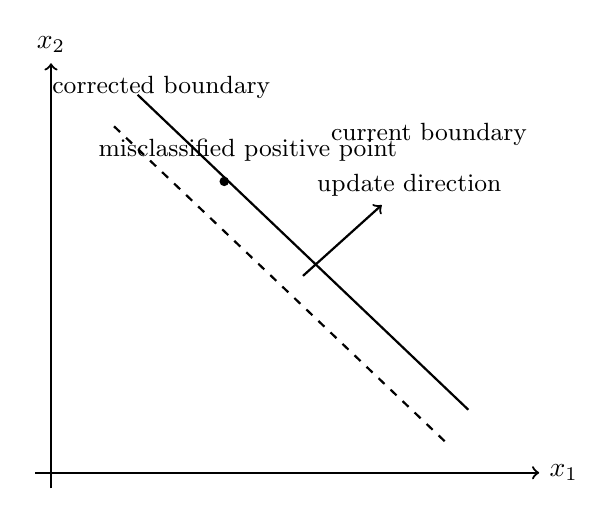
\begin{tikzpicture}[scale=1, every node/.style={align=center}]
    \draw[->, thick] (-0.2,0) -- (6.2,0) node[right] {$x_1$};
    \draw[->, thick] (0,-0.2) -- (0,5.2) node[above] {$x_2$};

    \draw[thick] (1.1,4.8) -- (5.3,0.8);
    \node at (4.8,4.3) {\small current boundary};

    \filldraw (2.2,3.7) circle (1.5pt);
    \node at (2.5,4.1) {\small misclassified positive point};

    \draw[->, thick] (3.2,2.5) -- (4.2,3.4);
    \node at (4.55,3.65) {\small update direction};

    \draw[dashed, thick] (0.8,4.4) -- (5.0,0.4);
    \node at (1.4,4.9) {\small corrected boundary};
\end{tikzpicture}
\caption{A perceptron update after a misclassified positive example. The update moves the separator so that the mistaken example becomes more likely to lie on the correct side.}
\end{figure}

\subsection*{The perceptron convergence theorem}

The perceptron is one of the first examples in machine learning where a simple algorithm admits a clean mathematical guarantee.

\begin{theorem}[Perceptron convergence]
Let $\{(x_i,y_i)\}_{i=1}^n$ with $y_i\in\{-1,1\}$ be linearly separable. Assume there exist a unit vector $u$ and a margin $\gamma>0$ such that
\[
y_i\,u^\top x_i \ge \gamma
\quad \text{for all } i,
\]
and assume $\|x_i\|\le R$ for all $i$. Then the perceptron algorithm, initialized at $w_0=0$, makes at most
\[
\left(\frac{R}{\gamma}\right)^2
\]
mistakes before it finds a separating hyperplane.
\end{theorem}

\begin{proof}
Suppose the algorithm makes $M$ mistakes. Let $w_t$ denote the weight vector after the $t$th mistake, with $w_0=0$.

At a mistake on example $(x_i,y_i)$, the update is
\[
w_{t+1}=w_t+y_i x_i.
\]
Taking inner product with $u$ gives
\[
u^\top w_{t+1}
=
u^\top w_t + y_i u^\top x_i
\ge
u^\top w_t + \gamma,
\]
because $y_i u^\top x_i\ge \gamma$ by assumption. Iterating this inequality over $M$ mistakes yields
\[
u^\top w_M \ge M\gamma.
\]

Now consider the squared norm. Since the update occurs only on a mistake, we have
\[
y_i(w_t^\top x_i+b_t)\le 0.
\]
Ignoring the bias for the moment and focusing on the weight vector, this implies in particular
\[
y_i w_t^\top x_i \le 0.
\]
Hence
\[
\|w_{t+1}\|^2
=
\|w_t+y_i x_i\|^2
=
\|w_t\|^2 + 2 y_i w_t^\top x_i + \|x_i\|^2
\le
\|w_t\|^2 + R^2.
\]
Iterating over $M$ mistakes gives
\[
\|w_M\|^2 \le M R^2.
\]

By the Cauchy--Schwarz inequality,
\[
M\gamma
\le
u^\top w_M
\le
\|u\|\,\|w_M\|
=
\|w_M\|
\le
\sqrt{M}\,R,
\]
because $\|u\|=1$. Therefore
\[
M\gamma \le \sqrt{M}\,R.
\]
If $M>0$, dividing by $\sqrt{M}\gamma$ gives
\[
\sqrt{M}\le \frac{R}{\gamma},
\]
so
\[
M\le \left(\frac{R}{\gamma}\right)^2.
\]
This proves the claim.
\end{proof}

The theorem is important for two reasons. First, it shows that learning can be proved to succeed under a geometric condition, namely linear separability with margin. Second, it clarifies the limitation of the perceptron: the guarantee depends on a setting in which a linear separator already exists.

\subsection*{Why nonlinear activations are essential}

The perceptron is already a composition of an affine map and a thresholding operation. But if we stack affine maps without nonlinearities, nothing fundamentally new happens.

\begin{proposition}[Composition of affine maps is affine]
Let
\[
A_1(x)=W_1x+b_1,
\qquad
A_2(z)=W_2z+b_2
\]
be affine maps. Then the composition $A_2\circ A_1$ is also affine:
\[
(A_2\circ A_1)(x)=W_2W_1x + (W_2b_1+b_2).
\]
Consequently, a multilayer network with only affine layers and no nonlinear activations is equivalent to a single affine map.
\end{proposition}

\begin{proof}
By direct substitution,
\[
(A_2\circ A_1)(x)
=
A_2(W_1x+b_1)
=
W_2(W_1x+b_1)+b_2
=
W_2W_1x + W_2b_1+b_2,
\]
which is again affine. Repeating the same argument across more layers shows that any finite composition of affine maps is affine.
\end{proof}

This proposition explains why nonlinearity is essential. Without it, depth collapses algebraically, and a deep stack of affine maps has no more expressive power than a single affine transformation.

\subsection*{Common activation functions}

A neural network inserts nonlinear activation functions between affine layers. If $z=Wx+b$, a common layer has the form
\[
h(x)=\sigma(z)=\sigma(Wx+b),
\]
where $\sigma$ is applied componentwise.

Some standard choices are:

\paragraph{Threshold activation.}
The perceptron uses
\[
\sigma(t)=\operatorname{sign}(t).
\]
This is conceptually simple but not differentiable in a way convenient for gradient-based training.

\paragraph{Sigmoid.}
\[
\sigma(t)=\frac{1}{1+e^{-t}}.
\]
This maps real numbers into $(0,1)$ and is historically important.

\paragraph{Hyperbolic tangent.}
\[
\sigma(t)=\tanh(t).
\]
This maps into $(-1,1)$ and is zero-centered.

\paragraph{ReLU.}
\[
\sigma(t)=\max\{0,t\}.
\]
This is simple, piecewise linear, and widely used in modern deep learning.

\paragraph{Leaky ReLU and related variants.}
These modify ReLU to allow a small negative slope when $t<0$.

The choice of activation influences both expressive power and trainability. Later sections will discuss this in more detail.

\subsection*{Multilayer feedforward networks}

With nonlinear activations in place, one can build genuine multilayer models.

\begin{definition}[Multilayer feedforward network]
A \emph{multilayer feedforward network} is a function obtained by composing affine maps and nonlinear activations in successive layers:
\[
h_1(x)=\sigma_1(W_1x+b_1),
\]
\[
h_2(x)=\sigma_2(W_2h_1(x)+b_2),
\]
and so on, until the final output
\[
f_\theta(x)=h_L(x).
\]
\end{definition}

The word \emph{feedforward} means that information flows from input to output without cycles. Each layer takes the previous layer's representation and transforms it into a new one.

\subsection*{Hidden layers as intermediate representations}

The intermediate variables
\[
z_1=h_1(x),\qquad z_2=h_2(x),\qquad \dots
\]
are called \emph{hidden representations}. They are “hidden” not in a mysterious sense, but simply because they are internal to the model rather than directly observed in the data.

This is where the link to Chapter 1 becomes explicit. A neural network is not just an output predictor. It is a machine for constructing a sequence of learned representations:
\[
x \mapsto z_1 \mapsto z_2 \mapsto \cdots \mapsto \hat y.
\]

One can therefore interpret hidden layers as learned feature maps,
\[
\phi_{\theta_1}(x)=z_k,
\]
followed by a predictor acting on those features.

\subsection*{A failure case: XOR}

The limitations of single-layer perceptrons are visible in the classical XOR example. Consider the four points
\[
(0,0),\ (0,1),\ (1,0),\ (1,1),
\]
with labels
\[
0,\ 1,\ 1,\ 0
\]
respectively. No single hyperplane can separate the positive and negative points correctly.

\begin{figure}[tbp]
\centering
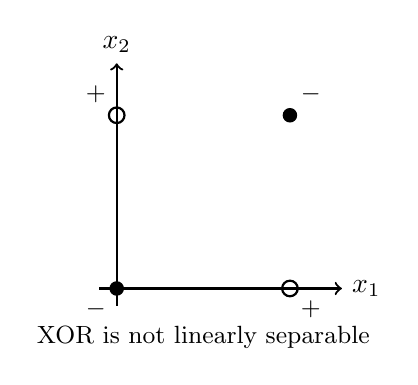
\begin{tikzpicture}[scale=2.2, every node/.style={align=center}]
    \draw[->, thick] (-0.1,0) -- (1.3,0) node[right] {$x_1$};
    \draw[->, thick] (0,-0.1) -- (0,1.3) node[above] {$x_2$};

    \filldraw (0,0) circle (1.1pt);
    \filldraw (1,1) circle (1.1pt);
    \draw[thick] (0,1) circle (0.045);
    \draw[thick] (1,0) circle (0.045);

    \node at (-0.12,-0.12) {\small $-$};
    \node at (1.12,1.12) {\small $-$};
    \node at (-0.12,1.12) {\small $+$};
    \node at (1.12,-0.12) {\small $+$};

    \node at (0.5,-0.28) {\small XOR is not linearly separable};
\end{tikzpicture}
\caption{The XOR pattern cannot be separated by a single hyperplane, so it cannot be represented by a single-layer perceptron. This motivates multilayer networks and nonlinear hidden representations.}
\end{figure}

The XOR example matters pedagogically because it shows that the limitation of the perceptron is not only quantitative but structural. Some simple logical patterns require hidden layers.

\subsection*{Composition as the central structural idea}

We can now state the main lesson of the section.

A neural network is a compositional model:
\[
f_\theta
=
h_L \circ h_{L-1} \circ \cdots \circ h_1.
\]
Each layer transforms one representation into another. The perceptron is the simplest instance of this idea. Multilayer networks generalize it by allowing repeated learned transformations, and nonlinear activations ensure that these transformations do not collapse into a single affine map.

So the real content of neural networks is not just “many parameters.” It is the structured composition of simple maps into increasingly expressive representation-building systems.

\commonconfusion{The perceptron is not just a historical curiosity. It is the first mathematically clean example of a learned classifier, and its convergence theorem is an important anchor result. At the same time, the success of modern deep learning does not come from stacking linear predictors alone. Without nonlinear activations, depth collapses to a single affine map, so the key issue is learned nonlinear composition, not mere repetition of matrix multiplication.}

\whattoremember{A perceptron is a halfspace classifier of the form $\operatorname{sign}(w^\top x+b)$, and the perceptron algorithm updates the weights only on mistakes. If the data are linearly separable with margin $\gamma$ and bounded norm $R$, the perceptron makes at most $(R/\gamma)^2$ mistakes. This gives Chapter 2 its first theorem-level anchor. The theorem also clarifies the limits of single-layer linear threshold models. To move beyond those limits, neural networks introduce nonlinear activations and hidden layers, turning learning into the composition of multiple trainable representation maps.}

\subsection*{Exercises}

\begin{exercise}
Run the perceptron algorithm by hand on the following dataset in $\mathbb R^2$:
\[
x_1=(1,1),\ y_1=1,
\qquad
x_2=(-1,-1),\ y_2=-1.
\]
Start from $w_0=0$, $b_0=0$, process the examples cyclically, and compute the first few updates until the dataset is classified correctly.
\end{exercise}

\begin{exercise}
Show that the bias term can be absorbed into the weight vector by augmenting the input with a constant $1$. More precisely, prove that
\[
w^\top x+b = \tilde w^\top \tilde x
\]
for suitable augmented vectors $\tilde w$ and $\tilde x$.
\end{exercise}

\begin{exercise}
Explain why the XOR labeling of the four points
\[
(0,0),\ (0,1),\ (1,0),\ (1,1)
\]
is not linearly separable.
\end{exercise}

\begin{exercise}
Prove directly that the composition of three affine maps is affine.
\end{exercise}

\begin{exercise}
Why does the proposition on affine composition show that nonlinear activations are essential in deep learning?
\end{exercise}

\begin{exercise}
Consider a perceptron $f(x)=\operatorname{sign}(w^\top x+b)$. What geometric object is defined by the equation
\[
w^\top x+b=0?
\]
How does the sign of $w^\top x+b$ determine the prediction?
\end{exercise}

\subsection*{Notes and references}

This section introduces the perceptron as the simplest neural-network-style classifier and uses it to establish the chapter's first major mathematical result: the perceptron convergence theorem. The perceptron is valuable not only historically but conceptually, because it shows how geometry, optimization, and classification already interact in a simple model. The section then explains why single-layer linear threshold models are not enough and why nonlinear activations and hidden layers are necessary. This opens the path to viewing neural networks as compositional systems for learned representation building rather than as mere collections of parameters.